\documentclass[a4paper, 12pt]{report}		% general format

%%%% Charset
\usepackage{cmap}							% make PDF files searchable and copyable
\usepackage[utf8]{inputenc}					% accept different input encodings
\usepackage[T2A]{fontenc}					% russian font
\usepackage[russian]{babel}					% multilingual support (T2A)

%%%% Graphics
\usepackage[dvipsnames]{xcolor}			% driver-independent color extensions
\usepackage{graphicx}						% enhanced support for graphics
\usepackage{wrapfig}						% pro­duces fig­ures which text can flow around

%%%% Math
\usepackage{amsmath}						% Amer­i­can Math­e­mat­i­cal So­ci­ety (AMS) math fa­cil­i­ties
\usepackage{amsfonts}						% fonts from the AMS
\usepackage{amssymb}						% additional math symbols

%%%% Ty­po­grapy (don't forget about cm-super)
\usepackage{microtype}						% sublim­i­nal re­fine­ments to­wards ty­po­graph­i­cal per­fec­tion
\linespread{1.3}							% line spacing
\usepackage[left=2.5cm, right=1.5cm, top=2.5cm, bottom=2.5cm]{geometry}
\setlength{\parindent}{0pt}					% we don't want any paragraph indentation
\renewcommand{\chaptername}{}

%%%% Other
\usepackage{hyperref}							% ver­ba­tim with URL-sen­si­tive line breaks
%\DeclareUnicodeCharacter{00A0}{~}
\usepackage{float}

%------------------------------------------------------------------------------
\usepackage{listings}						% type­set source code list­ings

% Цвета для кода
\definecolor{string}{HTML}{101AF9}			% цвет строк в коде
\definecolor{comment}{HTML}{3F7F5F}		% цвет комментариев в коде
\definecolor{keyword}{HTML}{5F1441}		% цвет ключевых слов в коде
\definecolor{morecomment}{HTML}{8000FF}	% цвет include и других элементов в коде
\definecolor{captiontext}{HTML}{FFFFFF}	% цвет текста заголовка в коде
\definecolor{captionbk}{HTML}{999999}		% цвет фона заголовка в коде
\definecolor{bk}{HTML}{FFFFFF}				% цвет фона в коде
\definecolor{frame}{HTML}{999999}			% цвет рамки в коде

% Настройки отображения кода
\lstset{
	language=C++,							% Язык кода по умолчанию
	morekeywords={*,...},					% если хотите добавить ключевые слова, то добавляйте
	% Цвета
	keywordstyle=\color{keyword}\ttfamily\bfseries,
	stringstyle=\color{string}\ttfamily,
	commentstyle=\color{comment}\ttfamily\itshape,
	morecomment=[l][\color{morecomment}]{\#},
	% Настройки отображения
	breaklines=true,						% Перенос длинных строк
	basicstyle=\ttfamily\footnotesize,		% Шрифт для отображения кода
	backgroundcolor=\color{bk},				% Цвет фона кода
	%frame=lrb,xleftmargin=\fboxsep,xrightmargin=-\fboxsep, % Рамка, подогнанная к заголовку
	frame=tblr								% draw a frame at all sides of the code block
	rulecolor=\color{frame},				% Цвет рамки
	tabsize=2,								% tab space width
	showstringspaces=false,					% don't mark spaces in strings
	% Настройка отображения номеров строк. Если не нужно, то удалите весь блок
	numbers=left,							% Слева отображаются номера строк
	stepnumber=1,							% Каждую строку нумеровать
	numbersep=5pt,							% Отступ от кода
	numberstyle=\small\color{black},		% Стиль написания номеров строк
	% Для отображения русского языка
	extendedchars=true,
    literate=
        {Ö}{{\"O}}1                    {Ä}{{\"A}}1                    {Ü}{{\"U}}1
        {ß}{{\ss}}1                    {ü}{{\"u}}1                    {ä}{{\"a}}1
        {ö}{{\"o}}1                    {~}{{\textasciitilde}}1        {а}{{\selectfont\char224}}1
        {б}{{\selectfont\char225}}1    {в}{{\selectfont\char226}}1    {г}{{\selectfont\char227}}1
        {д}{{\selectfont\char228}}1    {е}{{\selectfont\char229}}1    {ё}{{\"e}}1
        {ж}{{\selectfont\char230}}1    {з}{{\selectfont\char231}}1    {и}{{\selectfont\char232}}1
        {й}{{\selectfont\char233}}1    {к}{{\selectfont\char234}}1    {л}{{\selectfont\char235}}1
        {м}{{\selectfont\char236}}1    {н}{{\selectfont\char237}}1    {о}{{\selectfont\char238}}1
        {п}{{\selectfont\char239}}1    {р}{{\selectfont\char240}}1    {с}{{\selectfont\char241}}1
        {т}{{\selectfont\char242}}1    {у}{{\selectfont\char243}}1    {ф}{{\selectfont\char244}}1
        {х}{{\selectfont\char245}}1    {ц}{{\selectfont\char246}}1    {ч}{{\selectfont\char247}}1
        {ш}{{\selectfont\char248}}1    {щ}{{\selectfont\char249}}1    {ъ}{{\selectfont\char250}}1
        {ы}{{\selectfont\char251}}1    {ь}{{\selectfont\char252}}1    {э}{{\selectfont\char253}}1
        {ю}{{\selectfont\char254}}1    {я}{{\selectfont\char255}}1    {А}{{\selectfont\char192}}1
        {Б}{{\selectfont\char193}}1    {В}{{\selectfont\char194}}1    {Г}{{\selectfont\char195}}1
        {Д}{{\selectfont\char196}}1    {Е}{{\selectfont\char197}}1    {Ё}{{\"E}}1
        {Ж}{{\selectfont\char198}}1    {З}{{\selectfont\char199}}1    {И}{{\selectfont\char200}}1
        {Й}{{\selectfont\char201}}1    {К}{{\selectfont\char202}}1    {Л}{{\selectfont\char203}}1
        {М}{{\selectfont\char204}}1    {Н}{{\selectfont\char205}}1    {О}{{\selectfont\char206}}1
        {П}{{\selectfont\char207}}1    {Р}{{\selectfont\char208}}1    {С}{{\selectfont\char209}}1
        {Т}{{\selectfont\char210}}1    {У}{{\selectfont\char211}}1    {Ф}{{\selectfont\char212}}1
        {Х}{{\selectfont\char213}}1    {Ц}{{\selectfont\char214}}1    {Ч}{{\selectfont\char215}}1
        {Ш}{{\selectfont\char216}}1    {Щ}{{\selectfont\char217}}1    {Ъ}{{\selectfont\char218}}1
        {Ы}{{\selectfont\char219}}1    {Ь}{{\selectfont\char220}}1    {Э}{{\selectfont\char221}}1
        {Ю}{{\selectfont\char222}}1    {Я}{{\selectfont\char223}}1    {і}{{\selectfont\char105}}1
        {ї}{{\selectfont\char168}}1    {є}{{\selectfont\char185}}1    {ґ}{{\selectfont\char160}}1
        {І}{{\selectfont\char73}}1     {Ї}{{\selectfont\char136}}1    {Є}{{\selectfont\char153}}1
        {Ґ}{{\selectfont\char128}}1
}

% Для настройки заголовка кода
\usepackage{caption}
\DeclareCaptionFont{white}{\color{сaptiontext}}
\DeclareCaptionFormat{listing}{\parbox{\linewidth}{\colorbox{сaptionbk}{\parbox{\linewidth}{#1#2#3}}\vskip-4pt}}
%\captionsetup[lstlisting]{format=listing,labelfont=white,textfont=white}
\renewcommand{\lstlistingname}{Листинг} % Переименование Listings в нужное именование структуры

%------------------------------------------------------------------------------
\begin{document}

\begin{titlepage}

%----------------------------------------------------------------------------------------
%	HEADING SECTIONS
%----------------------------------------------------------------------------------------
\begin{center} % Center everything
Федеральное государственное автономное образовательное \\
учреждение высшего образования \\[0.4cm]

\includegraphics[scale=0.8]{res/SPbPU-logo} \\[0.4cm]
Институт компьютерных наук и технологий \\*
Высшая школа интеллектуальных систем и суперкомпьютерных технологий
\end{center}

\vspace{3cm}

%----------------------------------------------------------------------------------------
%	TITLE SECTION
%----------------------------------------------------------------------------------------
\begin{center} % Center everything
\textbf{Отчёт по лабораторному практимуму N1}\\
по дисциплине "Цифровые ресурсы в научных исследованиях" \\
по теме "Распределенные реестры (блокчейн) - \\ новые концепции и технологии последних лет" \\*
\end{center}

\vspace{3cm}
 
%----------------------------------------------------------------------------------------
%	AUTHOR SECTION
%----------------------------------------------------------------------------------------
\begin{flushleft}
Выполнил студент гр. 3540901/21501 \hspace{3cm} $\underset{\text{(подпись)}}{\underline{\hspace{3cm}}}$ С.А.Мартынов\\[0.5cm]
Преподаватель \hspace{7.25cm} $\underset{\text{(подпись)}}{\underline{\hspace{3cm}}}$ Е.Н.Бендарская\\[0.5cm]
\hspace{10.2cm} «\underline{\hspace{1cm}}» \underline{\hspace{3cm}} 2022 г.
\end{flushleft}

\vfill % Fill the rest of the page with whitespace

%----------------------------------------------------------------------------------------
%	DATE SECTION
%----------------------------------------------------------------------------------------
\begin{center}
Санкт-Петербург\\
2022
\end{center}

\end{titlepage}

\setcounter{page}{2}                            % inclide the title page
\tableofcontents
%\input{text}                                 % inclide the main text
%\newpage
\section*{}
\addcontentsline{toc}{section}{List of sources}

\begin{thebibliography}{00}

% Use: \cite{label1}
\bibitem{label1} text

\end{thebibliography}                              % inclide the list of sources

\chapter*{Задание 1. Ключевые слова}
\addcontentsline{toc}{chapter}{Задание 1. Ключевые слова}

\textbf{Задание:} сформулировать основные ключевые слова и словосочетания для выполнения первичного информационного запроса на русском языке по теме аналитического отчета. Записать ключевые слова и словосочетания в порядке релевантности. Выполнить поиск по всем ключевым словам и словосочетаниям, используемым как в одном поисковом запросе, так и по-отдельности, а провести поиск непосредственно по названию темы аналитического отчета. Провести первичную оценку результатов поиска путем выставления оценки от 1 до 10 степени релевантности полученных результатов для каждого запроса и представить их в отчете.

Не имя чёткого определения концепции "последних лет" буду ориентировать на публикации за последние 5 лет.

\section*{Список ключевых слов}
\addcontentsline{toc}{section}{Список ключевых слов}

Список ключевых слов сформирован на основе заявленной темы и дополнен имеющимися знаниями о предметной области
\begin{itemize}
\item распределённый реестр
\item блокчейн
\item консенсус
\item доказательство работы
\item доказательство владения
\end{itemize}

\section*{Поиск по словам и словосочетаниям}
\addcontentsline{toc}{section}{Поиск по словам и словосочетаниям}

В качестве основной поисковой системы был выбран \href{https://scholar.google.com/}{Google Scholar}. Для оценки результатов поиска будут анализироваться заголовки нескольких страниц по самым верхним ссылкам из списка результатов.

\subsection*{Поисковый запрос: Распределённый реестр}

\begin{enumerate}
\item \href{https://elibrary.ru/item.asp?id=44065996}{Анализ практической реализации технологии распределённого реестра}\\
В данной статье рассмотрена тенденция развития технологии распределённого реестра с течением времени, наиболее эффективные и перспективные виды распределённых реестров, их достоинства и недостатки. Среди ключевых слов заявлены: блокчейн, распределенный реестр, децентрализация, база данных, консенсус, смарт-контракт, криптография. Материал 2020 года, подподает под критерий свежести.\\
Оценка: 10/10.
\item \href{https://elibrary.ru/item.asp?id=44086179}{Распределенный реестр как технологическая основа децентрализованной системы финансов}\\
Метериал хуже анотирован в сравнении с предыдущей ссылкой, однако заявленная тема выглядит интересной. Материал 2020 года, подподает под критерий свежести.\\
Оценка: 6/10.
\item \href{https://cyberleninka.ru/article/n/tehnologii-raspredelyonnogo-reestra-i-zaschita-dokumentooborota-sudebnoy-sistemy}{Технологии распределённого реестра и защита документооборота судебной системы}\\
В документе приводится обоснование возможности создания судебной информационной системы документооборота на блокчейн-платформе, решения задачи обеспечения открытости сервиса для пользователей и поддержания высокой степени защищённости документальных данных всех участников судебного процесса на всем его протяжении. Среди ключевых слов заявлены: Судебная система, документооборот, блокчейн-сеть, технология блокчейн, электронное делопроизводство, распределенная база данных, система управления базой данных, хеш-функции, алгоритмы шифрования сети и пр. Материал 2020 года, подподает под критерий свежести.\\
Оценка: 8/10.
\end{enumerate}

\subsection*{Поисковый запрос: Блокчейн}

\begin{enumerate}
\item \href{https://cyberleninka.ru/article/n/blokcheyn-kak-kommunikatsionnaya-osnova-formirovaniya-tsifrovoy-ekonomiki-preimuschestva-i-problemy}{Блокчейн как коммуникационная основа формирования цифровой экономики: преимущества и проблемы}\\
В обзорной статье представлен анализ развития использования технологий распределенного реестра (блокчейн) в различных сферах социально-экономической жизни общества. Среди ключевых слов заявлены: прикладные информационные технологии, блокчейн, государственные информационные системы, государственное управление. Материал 2017 года, подподает под критерий свежести.\\
Оценка: 6/10.
\item \href{https://books.google.ru/books?hl=en&lr=&id=sP9CDwAAQBAJ&oi=fnd&pg=PT2&dq=%D0%B1%D0%BB%D0%BE%D0%BA%D1%87%D0%B5%D0%B9%D0%BD&ots=LGrkyFIDm_&sig=vSRGShqVEHSKbplbfM9LnVQWCeA&redir_esc=y#v=onepage&q=%D0%B1%D0%BB%D0%BE%D0%BA%D1%87%D0%B5%D0%B9%D0%BD&f=false}{Блокчейн: Как это работает и что ждет нас завтра}\\
Полноценная книга по истории развития блокчейн. Материал 2017 года, подподает под критерий свежести.\\
Оценка: 6/10.
\item \href{https://books.google.ru/books?hl=en&lr=&id=5peUDwAAQBAJ&oi=fnd&pg=PT3&dq=%D0%B1%D0%BB%D0%BE%D0%BA%D1%87%D0%B5%D0%B9%D0%BD&ots=pDls9WbrfK&sig=LvwOfXUGtqzJQScVAYn0YZqrNYQ&redir_esc=y#v=onepage&q=%D0%B1%D0%BB%D0%BE%D0%BA%D1%87%D0%B5%D0%B9%D0%BD&f=false}{Блокчейн. Схема новой экономики}\\
Книга об отображении возможностей валютного и финансового рынка на возможности блокчейн. Материал 2022 года, подподает под критерий свежести.\\
Оценка: 6/10.
\end{enumerate}

\subsection*{Поисковый запрос: Консенсус}

\begin{enumerate}
\item \href{https://economics.hse.ru/data/2011/02/14/1208909692/2010%20%D0%9C%D0%AD%D0%9C%D0%9E.pdf}{Вашингтонский консенсус: пейзаж после битв}\\
Материал 2010-го года на постороннюю тему (политика, история, экономика).\\
Оценка: 1/10.
\item \href{https://cyberleninka.ru/article/n/maastrihtskiy-konsensus-5-analiticheskiy-obzor-polozheniy}{Маастрихтский консенсус-5: аналитический обзор положений}\\
Материал 2017 года, но на постароннюю тему (медицина).\\
Оценка: 1/10.
\item \href{https://elibrary.ru/item.asp?id=26226720}{Политический консенсус. Теория и практика}\\
Материал 1997 года на постраннюю тему (политика).\\
Оценка: 1/10.
\end{enumerate}

\subsection*{Поисковый запрос: Доказательство работы}

\begin{enumerate}
\item \href{https://iling-ran.ru/library/grammar_theory_group/itg3.pdf#page=27}{Седьмое доказательство реальности ирреалиса}\\
Материал не релевантен, 2004 год.\\
Оценка: 1/10.
\item \href{https://cyberleninka.ru/article/n/elektronnye-dokazatelstva-v-normativnoy-sisteme-ugolovno-protsessualnyh-dokazatelstv}{Электронные доказательства в нормативной системе уголовно-процессуальных доказательств}\\
Материал 2019 года, но на постароннюю тему.\\
Оценка: 1/10.
\item \href{https://s.fundamental-research.ru/pdf/2008/3/1.pdf}{Ошибочное доказательство Уайлса великой теоремы Ферма}\\
Материал не релевантен.\\
Оценка: 1/10.
\end{enumerate}

\subsection*{Поисковый запрос: Доказательство владения}

\begin{enumerate}
\item \href{https://cyberleninka.ru/article/n/suschnost-kriptovalyut-deskriptivnyy-i-sravnitelnyy-analiz}{Сущность криптовалют: дескриптивный и сравнительный анализ}\\
Систематизация существующих в литературе и у международных и национальных организаций регуляторов взглядов на понятие криптовалюты, анализ ее экономической сущности и места в современной денежно-финансовой системе, 2019 год.\\
Оценка: 6/10.
\item \href{https://journal.altstu.ru/media/f/old2/pv2012_2_1/pdf/061sabanov.pdf}{Требования к системам аутентификации по уровням строгости}\\
Материал описывает фундаментальные вопросы и опубликован в 2012-м году, не подходит под критерий актуальности.\\
Оценка: 3/10.
\item \href{https://static.freereferats.ru/_avtoreferats/01002740942.pdf}{Владение как необходимое условие возникновения и осуществления вещных прав}\\
Материал не релевантен, 2004 год.\\
Оценка: 1/10.
\end{enumerate}

\subsection*{Поисковый запрос включает все поисковые слова}

\begin{enumerate}
\item \href{https://elibrary.ru/item.asp?id=44065996}{Анализ практической реализации технологии распределённого реестра}\\
Эта ссылка уже была представлена ранее.\\
Оценка: 10/10.
\item \href{https://cyberleninka.ru/article/n/blokcheyn-i-raspredelennye-reestry-kak-vidy-baz-dannyh}{Блокчейн и распределенные реестры как виды баз данных}\\
Статья раскрывает основные положения и некоторые технические особенности, лежащие в основе технологии распределенного реестра, необходимые для понимания возможности ее применения в различных областях экономики. Среди ключевых слов заявлены: блокчейн, технология распределенного реестра, базы данных, криптовалюты. Материал 2018 года, подподает под критерий свежести.\\
Оценка: 8/10.
\item \href{https://cyberleninka.ru/article/n/model-ustoychivogo-raspredelennogo-reestra-dlya-analiza-bezopasnosti-mnogomernogo-blokcheyna}{Модель устойчивого распределенного реестра для анализа безопасности многомерного блокчейна}\\
Рассмотрена задача построения модели устойчивого распределенного реестра, предназначенной для доказательства безопасности многомерного блокчейна. К модели предъявляется ряд требований, наиболее существенными из которых являются совместимость с существующими моделями и поддержка внешних транзакций. Среди ключевых слов заявлены: блокчейн, устойчивый распределенный реестр, многомерный блокчейн, фреймворк универсальной композиции, механизм достижения консенсуса, транзакции, доказательство безопасности. Материал 2021 года, подподает под критерий свежести.\\
Оценка: 9/10.
\end{enumerate}

\subsection*{Поиск по названию темы аналитического отчета}

\begin{enumerate}
\item \href{https://elibrary.ru/item.asp?id=44236813}{Технология блокчейн как драйвер цифровой экономики}\\
В статье проводится исследование перспектив технологии блокчейн в настоящее время. Предмет исследования - трансформирующий потенциал децентрализованных приложений. Цель статьи - на основе анализа возможностей реализованных распределенных реестров выявить качественные отличия технологии блокчейн от традиционных подходов и инструментов автоматизации бизнес-процессов. В качестве иллюстрации предлагается пример трансформации традиционного бизнес-процесса с помощью технологии блокчейн. Ключевые слова: биткоин, криптовалюта, блокчейн, распределенные реестры, децентрализованные приложения, распределенные системы, цифровая экономика, информационно-коммуникационные технологии. Материал 2020 года.\\
Оценка: 8/10.
\item \href{https://cyberleninka.ru/article/n/primenenie-tehnologiy-raspredelennogo-reestra-blockchain-v-elektroenergeticheskih-sistemah}{Применение технологий распределенного реестра (blockchain) в электроэнергетических системах}\\
Технология распределённого реестра обеспечивает распределенные вычисления, безопасную среду для взаимодействия участников в сети и надежное хранение информации. Ключевые слова: blockchain, smart grid, distributed computing, распределенный реестр. Публикация 2020 года.\\
Оценка: 7/10.
\item \href{https://books.google.ru/books?id=R5aRDwAAQBAJ&lpg=PT2&ots=K3b2kZeO2J&dq=%D0%A0%D0%B0%D1%81%D0%BF%D1%80%D0%B5%D0%B4%D0%B5%D0%BB%D0%B5%D0%BD%D0%BD%D1%8B%D0%B5%20%D1%80%D0%B5%D0%B5%D1%81%D1%82%D1%80%D1%8B%20(%D0%B1%D0%BB%D0%BE%D0%BA%D1%87%D0%B5%D0%B9%D0%BD)%20%D0%BD%D0%BE%D0%B2%D1%8B%D0%B5%20%D0%BA%D0%BE%D0%BD%D1%86%D0%B5%D0%BF%D1%86%D0%B8%D0%B8%20%D0%B8%20%D1%82%D0%B5%D1%85%D0%BD%D0%BE%D0%BB%D0%BE%D0%B3%D0%B8%D0%B8%20%D0%BF%D0%BE%D1%81%D0%BB%D0%B5%D0%B4%D0%BD%D0%B8%D1%85%20%D0%BB%D0%B5%D1%82&lr&pg=PT2#v=onepage&q&f=false}{Блокчейн на практике}\\
Весьма подробная книга, но начального уровня. Опубликована в 2019 году.\\
Оценка: 6/10.
\end{enumerate}

\chapter*{Задание 2. Оценка качества представленных ссылок}
\addcontentsline{toc}{chapter}{Задание 2. Оценка качества представленных ссылок}

\textbf{Задание:} оценить качество и количество представленных ссылок для лучшего варианта поискового запроса - оценка степени удовлетворенности качеством представленных источников от 1 (совсем не соответствует ожиданиям) до 10 (именно то, что ожидалось найти) и оценка достаточности представленных источников от 1 (очень мало) до 10 (очень много), и на этом основании выполнить уточнение информационного запроса – дополнение ключевых слов (исключение ключевых слов), расширение ключевых словосочетаний синонимами и т.д. Провести первичную оценку результатов поиска путем выставления оценки от 1 до 10 степени релевантности полученных результатов для каждого запроса и представить их в отчете.

При первичном анализе, сразу обращают на себя внимание следующие факты:
\begin{enumerate}
\item Более общие запросы (распределённый реестр, блокчейн) давали более точные результаты, чем более конкретные запросы (доказательство работы, доказательство владения). Мы полагаем, что это может быть связано с тем, что "доказательства работы" и "доказательства владения" являются дословным переводом с английского языка и в научной литеретуре могут использоваться без перевода.
\item При поиске, мы практически не сталкивались с сильно устаревшими данными. Это говорит о том, что тема переживает бурное развитие, хотя и строится на основе фундаментальных механик (хешировании, шифровании, сетевом обмене).
\item Слово "консенсус" имеет слишком широкое применение в большом количестве предметных областей.
\item Слово "блокчейн" часто используется в материалах начального уровня, которые объясняют основы построения таких сетей, и стараются избегать рассмтрения путей решения для сложных проблем.
\item Часто можно встретить материалы на тему прикладного использования распределённых реестров, это является свидетельством того, что тема перешагнула академическую среду и имеет реальное применение.
\end{enumerate}

Достаточность материалов по любому из запросов на вызывает затруднений.

С точки зрения релевантости, наиболее полезными были следующие запросы (от более релевантного к менее):

\begin{enumerate}
\item Поисковый запрос, включавший все поисковые слова.
\item Поиск по слову "распределенный реестр".
\item Поиск по названию темы аналитического отчёта.
\end{enumerate}


\chapter*{Задание 3. Коррекция поискового запроса}
\addcontentsline{toc}{chapter}{Задание 3. Коррекция общего поискового запроса}

\textbf{Задание}: Сравнить набор ключевых слов из лучших найденных источников (представить в отчете) и использованных при выполнении поискового запроса. Сделать вывод о необходимости коррекции состава ключевых слов или формулировки общего поискового запроса.

\section*{Комбинация поисковых запросов}
\addcontentsline{toc}{section}{Комбинация поисковых запросов}

По итогам первичного анализа ссылок, попробуем скомбинировать широко применяемое слово "консенсус" с видами доказательств.

\subsection*{Поисковый запрос: Консенсус, Доказательство работы}

\begin{enumerate}
\item \href{https://cyberleninka.ru/article/n/suschnost-kriptovalyut-deskriptivnyy-i-sravnitelnyy-analiz}{Сущность криптовалют: дескриптивный и сравнительный анализ}\\
Ссылка рассматривалась выше.\\
Оценка: 6/10.
\item \href{https://elibrary.ru/item.asp?id=39323497}{Свойства механизмов консенсуса в технологии блокчейн}\\
В статье проанализированы механизмы достижения консенсуса в технологии блокчейн, возникшей как альтернатива традиционной технологии на основе распределенных баз данных, управляемых с помощью системы администрирования. Ключевые слова: блокчейн, майнер, биткойн, злоумышленник, механизм консенсуса, хеш-функция, биномиальное распределение вероятностей. Публикация 2019 года.\\
Оценка: 8/10.
\item \href{https://elibrary.ru/item.asp?id=37116587}{Анализ алгоритмов консенсуса}\\
В работе приведено описание существующих алгоритмов консенсуса в децентрализованной базе данных и их сравнение по таким параметрам, как масштабируемость, скорость работы, надежность. Сделаны выводы о практической применимости. Опубликована в 2019 году.\\
Оценка: 9/10.
\end{enumerate}

\subsection*{Поисковый запрос: Консенсус, Доказательство владения}

\begin{enumerate}
\item \href{https://elibrary.ru/item.asp?id=44236813}{Технология блокчейн как драйвер цифровой экономики}\\
В статье проводится исследование перспектив технологии блокчейн в настоящее время. Предмет исследования - трансформирующий потенциал децентрализованных приложений. Цель статьи - на основе анализа возможностей реализованных распределенных реестров выявить качественные отличия технологии блокчейн от традиционных подходов и инструментов автоматизации бизнес-процессов. В качестве иллюстрации предлагается пример трансформации традиционного бизнес-процесса с помощью технологии блокчейн. Ключевые слова: биткоин, криптовалюта, блокчейн, распределенные реестры, децентрализованные приложения, распределенные системы, цифровая экономика, информационно-коммуникационные технологии. Материал 2020 года.\\
Оценка: 8/10.
\item \href{https://elibrary.ru/item.asp?id=38568047}{Вопросы управления саморегулируемых организацийй (СРО) с использованием применения консенсуса доказательства полномочий (РОА)}\\
В статье рассматриваются вопросы применения распределенных реестров в саморегулируемых организациях. Рассматриваются основные преимущества и недостатки наиболее распространенных моделей консенсуса. Приведена модель применения консенсуса доказательства полномочий в саморегулируемых организациях. Рассмотрены основные компоненты такой системы и их реализация. Также рассмотрены основные правовые и технические проблемы реализации подобных систем. Публикация 2019 года.\\
Оценка: 9/10.
\item \href{https://cyberleninka.ru/article/n/blokcheyn-i-raspredelennye-reestry-kak-vidy-baz-dannyh}{Блокчейн и распределенные реестры как виды баз данных}\\
Ссылка рассматривалась выше.\\
Оценка: 8/10.
\end{enumerate}


\chapter*{Задание 4. Дополнительная поисковая система}
\addcontentsline{toc}{chapter}{Задание 4. Дополнительная поисковая система}

\textbf{Задание}: Выполнить п. 1-3 в еще одной (другой) поисковой системе. Сравнить полученные результаты и сформулировать выводы.

В качестве 2й платформы был выбран \href{https://library.spbstu.ru/ru/}{Информационно-библиотечный комплекс Политех}.

\section*{Поиск по исходному списку слов}
\addcontentsline{toc}{section}{Поиск по исходному списку слов}

\subsection*{Поисковый запрос: Распределённый реестр}

\href{https://ruslan.library.spbstu.ru/pwb/detail?db=ANALITS2005&id=RU%5CSPSTU%5Canalits2005%5C391759}{Распределенные реестры в цифровой экономике: база данных, технология или протокол?}\\
В статье представлен анализ концептуальных подходов к трактовке дефиниции "распределенный реестр" как основы инновационных финансово-расчетных инструментов. Предложена авторская интерпретация данного понятия. Систематизирована и дополнена классификация распределенных реестров как с позиции способа обмена, хранения и обработки информации на основе комплекса технологий. Публикация 2019 года.\\
Оценка: 6/10.

\subsection*{Поисковый запрос: Блокчейн}

\href{https://ruslan.library.spbstu.ru/pwb/detail?db=ANALITS2005&id=8c229831-1a03-4873-b151-28e250859458}{Разработка методики и комплекса программных средств для дистанционного электронного голосования на основе блокчейн-платформы Ethereum}\\
В работе предложена методика построения дистанционного электронного голосования. По структуре она аналогична традиционному способу голосования: используется тот же принцип и процессы. Подробно описан процесс дистанционного электронного голосования на основе блокчейн-платформы Ethereum. Показано, что полученные голоса надежно хранятся в блокчейн-сети Ethereum, а правильность адресации голоса выбранному кандидату всегда можно проверить в режиме реального времени. Материал 2017 года, подподает под критерий свежести.\\
Оценка: 6/10.

\subsection*{Поисковый запрос: Консенсус}

\href{https://ruslan.library.spbstu.ru/pwb/detail?db=ANALITS2005&id=RU%5CSPSTU%5Canalits2005%5C10209}{Консерватизм и либерализм: метаморфозы консенсуса}\\
Тема не релевантна.\\
Оценка: 1/10.

\subsection*{Поисковый запрос: Доказательство работы}

\href{https://ruslan.library.spbstu.ru/pwb/detail?db=ANALITS2005&id=RU%5CSPSTU%5Canalits2005%5C385225}{Организационно-педагогические условия формирования личности безопасного типа поведения у студентов через изучение дисциплины "Безопасность жизнедеятельности"}\\
Тема не релевантна.\\
Оценка: 1/10.

\subsection*{Поисковый запрос: Доказательство владения}

\href{https://ruslan.library.spbstu.ru/pwb/detail?db=ANALITS2005&id=RU%5CSPSTU%5Canalits2009%5C42785}{Комментарий судебного спора}\\
Систематизация существующих в литературе и у международных и национальных организаций регуляторов взглядов на понятие криптовалюты, анализ ее экономической сущности и места в Тема не релевантна.\\
Оценка: 1/10.
Всего один поисковый результат!

\subsection*{Поисковый запрос включает все поисковые слова}

Результатов нет!

\subsection*{Поиск по названию темы аналитического отчета}

Результатов нет!

\section*{Первичная оценка}
\addcontentsline{toc}{section}{Первичная оценка}

Полученные результаты значительно скромнее, чем результаты Google. По некоторым запросам результата нет вообще.

\section*{Коррекция поискового запроса}
\addcontentsline{toc}{section}{Коррекция поискового запроса}

Попробуем повторить тот же приём комбинирования слова "консенсус" с видами доказательств. Гипотеза в том, что из всего множество ответов на запрос по слову "консенсус" поисковая машина сможет подобрать те, которые наиболее близки теме распределённых реестров (как это было с Google)

\subsection*{Поисковый запрос: Консенсус, Доказательство работы}

Результатов нет!

\subsection*{Поисковый запрос: Консенсус, Доказательство владения}

Результатов нет!

\section*{Сравнение результатов}
\addcontentsline{toc}{section}{Сравнение результатов}

Поисковые возможности Google оказались значительно более мощными и предоставили гораздо больше релевантных материалов.

Возможно, причина в том, как именно осуществляется поиск: если Информационно-библиотечный комплекс Политех осуществляет поиск по заранее подготовленной мета-информации, то Гугл индексирует полностью весь материал, строит семантические связи и умеет работать с падежами и склонениями. Проверка этой гипотезы выходит за рамки данного исследования.

\chapter*{Задание 5. Расширенный поиск}
\addcontentsline{toc}{chapter}{Задание 5. Расширенный поиск}

\textbf{Задание}: Изучить возможности поисковых систем по работе с расширенным поиском. Использовать расширенный поиск – привести примеры выполненного расширенного поиска и оценить качество полученных результатов по сравнению с простым поисковым запросом. Сделать выводы.

\section*{Google Scholar}
\addcontentsline{toc}{section}{Google Scholar}

Окно расширенного поиска показано на рисунке 1.

\begin{figure}[H]
 \centering
 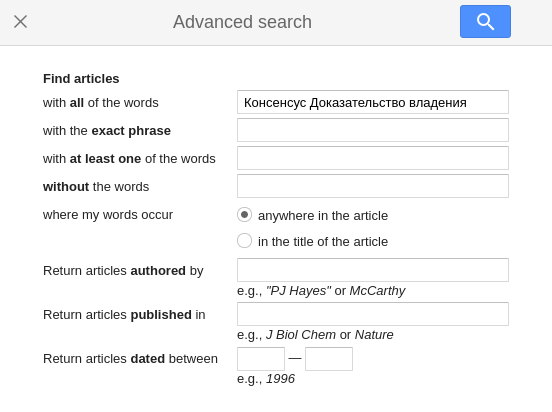
\includegraphics[scale=0.8]{res/src1}
 \caption{Расширенный поиск Google Scholar}
\end{figure}

Каждая строчка хорошо анотирована и имеет понятное назначение.

Кроме того, параметры поиска можно задавать прямо в поисковой строке. К примеру, "Консенсус Доказательство владения author:McCarthy source:Nature"

\section*{Информационно-библиотечный комплекс Политех}
\addcontentsline{toc}{section}{Информационно-библиотечный комплекс Политех}

Расширенный поиск Информационно-библиотечного комплекса Политех построен по двухуровневой системе. На первом шаге можно указать тип документа, и добавить условия используя обычные булевы операции (рисунок 2).

\begin{figure}[H]
 \centering
 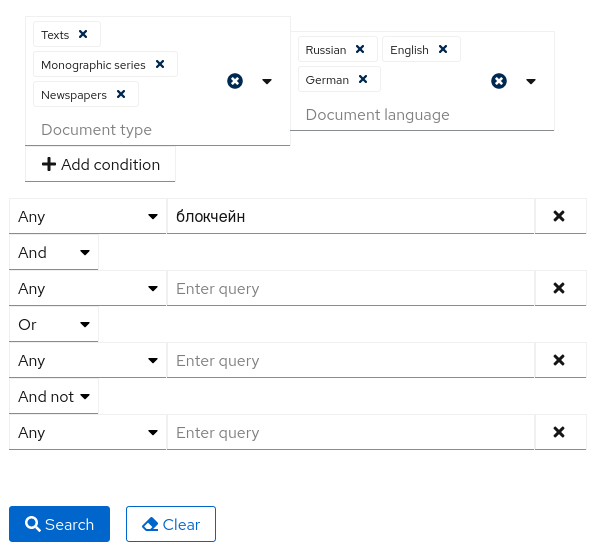
\includegraphics[scale=0.8]{res/src2}
 \caption{Окно поиска Информационно-библиотечного комплекса Политех}
\end{figure}

Сразу после поиска, появляется второй уровень, где можно провести дополнительную фильтрацию полученных результатов (рисунок 3).

\begin{figure}[H]
 \centering
 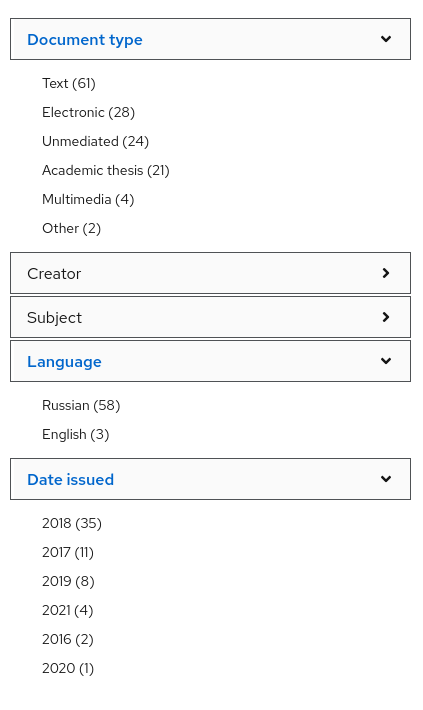
\includegraphics[scale=0.8]{res/src3}
 \caption{Фильтрация результатов поиска}
\end{figure}

\section*{Выводы}
\addcontentsline{toc}{section}{Выводы}

Предложенные варианты управления поисковыми запросами достаточно удобны, особенно если достаточно в этом практироваться (синтаксис усправляющих команд Google Scholar аналогичен синтаксису обычного Google Поиска). Для нашей задачи наиболее интересным критерием является отсечение по дате, т.к. нас интересуют материалы только за последние 5 лет. Однако на практике среди релевантных результатов устаревшие статьи появлялись на столько редко, что их ручной отсев не представляет никакой сложности.

\chapter*{Задание 6. Переработка текста}
\addcontentsline{toc}{chapter}{Задание 6. Переработка текста}

\textbf{Задание}: Выбрать из найденных источников наиболее релевантный и осуществить переработку первичного текста во вторичный, путем выполнения аннотирования с критической оценкой первоисточника и реферирования. Составить описательную аннотацию к тексту (описательная аннотация излагает, «о чем» написан первоисточник и лишь называет основные моменты содержания), составить реферативную аннотацию к тексту (реферативная аннотация, отражая основные вопросы содержания, в предельно сжатом виде передает также выводы по каждому из затронутых вопросов и по материалу в целом), составить аннотацию-резюме к тексту (аннотация-резюме характеризуется четкой передачей главного тематического содержания в предельно сжатом виде). Составить информативный реферат текста (не более 1/2 - 3/4 страницы).

Для работы выберем один из материалов, получивший 10 баллов по шкале релевантности: \href{https://elibrary.ru/item.asp?id=44065996}{Анализ практической реализации технологии распределённого реестра}

\section*{Описательная аннотация}
\addcontentsline{toc}{section}{Описательная аннотация}
% описательная аннотация излагает, «о чем» написан первоисточник и лишь называет основные моменты содержания
В статье содержится информация о нескольких основных алгоритмах достижения консенсуса и проводится сравнение их реализации.

\section*{Реферативная аннотация}
\addcontentsline{toc}{section}{Реферативная аннотация}
% отражая основные вопросы содержания, в предельно сжатом виде передает также выводы по каждому из затронутых вопросов и по материалу в целом
В статье происходит сравнение алгоритмов достижения консесуса в технологиях распределенного реестра на примере таких проектов, как Holochain и Radix, что демонстирует зрелость подхода для использования в разных секторах и отраслях промышленности.

\section*{Аннотация-резюме}
\addcontentsline{toc}{section}{Аннотация-резюме}
% характеризуется четкой передачей главного тематического содержания в предельно сжатом виде
Главной темой исследования является изучение алгоритмов достижения консесуса и сравнение достоинств и недостатков как традиционных (доказательство работы) так и более современных подходов (таких как доказательство доли или византийская отказоустойчивость).

\section*{Информативный реферат}
\addcontentsline{toc}{section}{Информативный реферат}
% представляет собой описание научной работы с указанием всех важных моментов реферируемого текста: предмета и цели, описание методов и средств, полученных выводов и их ценность. Состоит он из следующих частей:
%    - вводная с указанием полной информации об источнике : кто написал статью, когда опубликовали и где, тема и суть;
%    - основная часть с подробностями (что конкретно проводилось в числах, формулах, методах);
%    - заключение, содержащее итог научной работы по мнению автора статьи, важность проведенных исследований и дальнейшая перспектива в описываемой области.
Статья "Анализ практической реализации технологии распределённого реестра" была разработана коллективом авторов под руководством Сафарьян О.А. (к.т.н) и опубликована в сборнике научных статей 7-й Всероссийской научно-технической конференции "Прогрессивные технологии и процессы" (Курск, 2020).

Авторы работы подмечают, что современный тренд на переход к цифровой информации оставляет пространство для злоумышленников. Это хорошо видно на примере глобальной сети Интернет в которой скопилось много ненужной и недостоверной информации, а доступ к сети
зачастую анонимен и не защищён. Эти и многие другие проблемы можно решить с помощью технологии распределённого реестра. Сильной сторой такого подхода является отсутсвие централизованного узла, что делает многие операции значительно более дешёвыми, т.к. исключает необходимость привлекать третье (доверенное) лицо.

Информацию в распределённый реестр может вносить любой пользователь, что влечёт за собой необходимость проверки информацию на достоверность. Решением данной проблемы решается механизмом достижения консенсуса. Существует несколько основных алгоритмов достижения консенсуса.

\begin{itemize}
\item Доказательство работой (Proof-of-work, PoW).
\item Доказательство владения доли (Proof-of-stake, PoS)
\item Направленный ациклический граф (Directed Acyclic Graphs, DAG)
\item Византийская отказоустойчивость (Byzantine fault tolerance, BFT)
\item Делегированное доказательство владения доли (Delegated proof-of-stake, DPoS)
\item Направленный ациклический граф (Directed Acyclic Graphs, DAG)
\end{itemize}

Каждый подход имеет свои минусы и плюсы.

Holochain -- это платформа на основе распределенной сети с автономными возможностями для пользователей. Вместо поддержки единого консенсуса, распределенная хеш-таблица Holochain содержит отчет об основном виде и легитимности информации, предоставляемой отдельными блок-цепями. Это устраняет необходимость слежения за каждым действием в сети и потребность в глобальном консенсусе.

Еще один распределённого реестр Radix используют Логические Часы для валидации транзакций, которая достигается за счет запоминания последовательности транзакций для достижения консенсуса. Пропускная способность Radix составляет 20000 транзакций в секунду при 10 активных узлах.

Сравнение между технологиями распределенного реестра показывает, что эта идея уже прошла долгий путь цифровой революции. Проекты подобные Holochain и Radix выводят идею децентрализации на следующий уровень и демонстирует зрелость подхода для использования в разных секторах и отраслях промышленности.

\chapter*{Задание 7. Запрос на английском языке}
\addcontentsline{toc}{chapter}{Задание 7. Запрос на английском языке}

\textbf{Задание}: Выполнить п. 1-6 для информационного запроса на английском языке

\section*{Список ключевых слов}
\addcontentsline{toc}{section}{Список ключевых слов}

\begin{itemize}
\item distributed registry
\item blockchain
\item consensus
\item proof of work
\item proof of stake
\end{itemize}

\section*{Поиск по словам и словосочетаниям}
\addcontentsline{toc}{section}{Поиск по словам и словосочетаниям}

\subsection*{Поисковый запрос: distributed registry}

\textbf{Google Scholar}

\begin{enumerate}
\item \href{https://ieeexplore.ieee.org/abstract/document/5072554}{A recommender system for web services discovery in a distributed registry environment}\\
In this paper, the suitability of using recommendation techniques for Web service discovery in distributed registry environments is descussed. The architecture consists in structuring registries of Web services into groups. Material from 2009, does not meet the criteria of freshness.\\
Оценка: 1/10.
\item \href{https://elibrary.ru/item.asp?id=44086179}{Digital registry of professional competences of the population drawing on distributed registries and smart contracts technologies}\\
The proposed model presents the educational level and professional skills of each registered person as an education index (EI), which keeps track of all educational achievements and professional competencies of the participant over their lifetime. When calculating the EI, the authors also propose to consider ratings of the educational institutions responsible for the participant’s professional skills. 2018.\\
Оценка: 6/10.
\item \href{https://cyberleninka.ru/article/n/tehnologii-raspredelyonnogo-reestra-i-zaschita-dokumentooborota-sudebnoy-sistemy}{Ad-UDDI: An active and distributed service registry}\\
In SOA (Service Oriented Architecture), web service providers use service registries to publish services and requestors use registries to find them. The major current service registry specifications, UDDI (Universal Description, Discovery and Integration), has  some drawbacks. 2005.\\
Оценка: 1/10.
\end{enumerate}

\textbf{Информационно-библиотечный комплекс Политех}

Только 2 материала!

\begin{enumerate}
\item \href{https://ruslan.library.spbstu.ru/pwb/detail?db=EBOOKS&id=RU%5CSPSTU%5Cedoc%5C61996}{The management of business processes of the integrated structures on the principles of sharing of digital technology}\\
he purpose of the study is to substantiate the nature, features and possibilities of the joint use of distributed registry technologies and "big data" in the management of business processes of integrated structures. The study was conducted on the materials characterizing the development of this concept both in the whole world and its spread in the Russian economy. It is proved that for business it is possible to consider perspective Association of blockchain technologies and "big data" as there is an opportunity to model a large number of business processes. 2019.\\
Оценка: 3/10.
\item \href{https://ruslan.library.spbstu.ru/pwb/detail?db=EBOOKS&id=RU%5CSPSTU%5Cedoc%5C64106}{Models for integrating digital technologies into the international payment space}\\
The paper identifies four approaches to the organization of cooperation between countries in order to carry out cross-border settlement, which consider nine models of international cooperation depending on the configuration (centralized electronic or decentralized digital) of national and international payment and settlement systems. On the basis of the comparative analysis of the models parameters, the author chooses an option of inter-country cooperation in the financial sphere within the framework of the common digital payment space. It involves a digital settlements infrastructure, both at the national level and between countries. 2020.\\
Оценка: 2/10.
\end{enumerate}

\subsection*{Поисковый запрос: blockchain}

\textbf{Google Scholar}

\begin{enumerate}
\item \href{https://allquantor.at/blockchainbib/pdf/zheng2018blockchain.pdf}{Blockchain challenges and opportunities: A survey}\\
This paper gives the blockchain taxonomy, introduces typical blockchain consensus algorithms, reviews blockchain applications and discusses technical challenges as well as recent advances in tackling the challenges. Moreover, this paper also points out the future directions in the blockchain technology. 2018.\\
Оценка: 7/10.
\item \href{https://ieeexplore.ieee.org/abstract/document/8805074}{A survey of blockchain from the perspectives of applications, challenges, and opportunities}\\
 This paper presents a comparative study of the tradeoffs of blockchain and also explains the taxonomy and architecture of blockchain, provides a comparison among different consensus mechanisms and discusses challenges, including scalability, privacy, interoperability, energy consumption and regulatory issues. In addition, this paper also notes the future scope of blockchain technology. 2019.\\
Оценка: 9/10.
\item \href{https://ieeexplore.ieee.org/abstract/document/8760539}{A vademecum on blockchain technologies: When, which, and how}\\
In this paper, authors aim at providing the community with such a vademecum, while giving a general presentation of blockchain that goes beyond its usage in Bitcoin and surveying a selection of the vast literature that emerged in the last few years. They draw the key requirements and their evolution when passing from permissionless to permissioned blockchains, presenting the differences between proposed and experimented consensus mechanisms, and describing existing blockchain platforms. 2019.\\
Оценка: 9/10.
\end{enumerate}

\textbf{Информационно-библиотечный комплекс Политех}

\begin{enumerate}
\item \href{https://ruslan.library.spbstu.ru/pwb/detail?db=ANALITS2005&id=8c229831-1a03-4873-b151-28e250859458}{Methods and software complex development for remote electronic voting based on Ethereum blockchain platform}\\
In this work, a method for constructing a REV is proposed that solves these problems. It is similar in structure to the traditional voting method, using the same principle and processes. The Ethereum blockchain based REV process is described in detail. It was shown that received votes are securely stored in the Ethereum blockchain network, and the correctness of the vote addressing to the selected candidate can always be checked in real time. The description of smart contract algorithm that implements the transfer of vote from voter to candidate using transactions and determines the winner who received the highest number of votes was provided. 2021.\\
Оценка: 6/10.
\item \href{https://ruslan.library.spbstu.ru/pwb/detail?db=ANALITS2005&id=RU%5CSPSTU%5Canalits2005%5C349269}{Blockchain based decentralized public key infrastructure model}\\
The paper reviews the most commonly used public key infrastructures, provides their disadvantages. There is suggested a decentralized public key infrastructure model which excludes these disadvantages. Blockchain technology applying for public key infrastructure is proposed. The set of existing blockchain based public key infrastructure have been overviewed and analyzed in the context of the defined model. 2017.\\
Оценка: 6/10.
\item \href{https://ruslan.library.spbstu.ru/pwb/detail?db=ANALITS2005&id=RU%5CSPSTU%5Canalits2005%5C349543}{Cryptocurrency and blockchain technology in digital economy: development genesis}\\
The main historical events of the origin of cryptocurrencies are considered. The economic essence of digital money (Fiat) and cryptocurrencies is analyzed, their comparative characteristic is given. The features of state regulation of cryptocurrencies in Australia are studied. The analysis of legal regulation in the UK. The main stages of development of state regulation in China, the USA and Ukraine are investigated. Steps of legal regulation in the USA are considered. The main initiatives and proposals of the relative legal regulation of cryptocurrencies in the Russian Federation are studied in detail. SWOT analysis of cryptocurrencies was carried out. On the basis of the Genesis of the development of cryptocurrencies and blockchain technology, the problems of the digital economy are reflected, the directions of further research are shown. 2017.\\
Оценка: 5/10.
\end{enumerate}

\subsection*{Поисковый запрос: consensus}

\textbf{Google Scholar}

Большое количество результатов не подходящих по году издания! Пришлось добавить фильтрацию по дате в поисковый запрос.

\begin{enumerate}
\item \href{https://ieeexplore.ieee.org/abstract/document/8972381}{A survey of distributed consensus protocols for blockchain networks}\\
Among various core components, consensus protocol is the defining technology behind the security and performance of blockchain. From incremental modifications of Nakamoto consensus protocol to innovative alternative consensus mechanisms, many consensus protocols have been proposed to improve the performance of the blockchain network itself or to accommodate other specific application needs. In this survey, authors present a comprehensive review and analysis on the state-of-the-art blockchain consensus protocols. 2020.\\
Оценка: 10/10.
\item \href{https://www.sciencedirect.com/science/article/abs/pii/S0957417420302098}{A survey of blockchain consensus algorithms performance evaluation criteria}\\
To overview and provide a basis of comparison for further work, a set of incommensurable and conflicting performance evaluation criteria is identified and weighted by the pairwise comparison method. These criteria are classified into four categories including algorithms throughput, the profitability of mining, degree of decentralization and consensus algorithms vulnerabilities and security issues. Based on the proposed framework, the pros and cons of consensus algorithms are systematically analyzed and compared in order to provide a deep understanding of the existing research challenges and clarify the future study directions. 2020.\\
Оценка: 9/10.
\item \href{https://ieeexplore.ieee.org/abstract/document/9376868}{A comprehensive review of blockchain consensus mechanisms}\\
Analyzing 185 publications, ranging from academic journals to industry websites, it provides a comparative analysis of 130 consensus algorithms using a novel architectural classification. The distribution of the reviewed algorithms is analyzed in terms of the proposed classification and different application domains, along with the applicability of each class among the top 10 platforms in the most prominent blockchain application domains. Additional conclusions are drawn from the evolution of consensus mechanisms, and the analysis concludes envisaging future prospects for consensus as an important part of distributed ledger technology. 2021.\\
Оценка: 10/10.
\end{enumerate}

\textbf{Информационно-библиотечный комплекс Политех}

Так же пришлось использовать фильтрацию по дате публикации.

\begin{enumerate}
\item \href{https://ruslan.library.spbstu.ru/pwb/detail?db=EBOOKS&id=RU%5CSPSTU%5Cedoc%5C62081}{From precariatization to precarious work: theoretical understanding of paradigmatic concepts}\\
Analysis of Russian and foreign literature showed a lack of consensus regarding the interpretation of the concepts "employment precariatization" and "precarious work". Due to this, based on the principle of universality, we have described our views on the essence of the phenomena considered in the context of transformation processes in the sphere of social and labor relations. 2019.\\
Оценка: 1/10.
\item \href{https://ruslan.library.spbstu.ru/pwb/detail?db=EBOOKS&id=RU%5CSPSTU%5Cedoc%5C54944}{Polarity, balance of power and international relations theory: post-cold war and the 19th century compared}\\
Here, the author analyses different historic eras through a polarity lens, compares the way polarity is used in the French and US public discourses, and through careful examination, reaches the conclusion that polarity terminology as a theoretical concept is highly influenced by the Cold War context in which it emerged. The book is an important resource for students and researchers with a critical approach to Neorealism, and to those interested in the defining shifts the world went through during the last twenty five years. 2017.\\
Оценка: 1/10.
\item \href{https://ruslan.library.spbstu.ru/pwb/detail?db=ANALITS2005&id=RU%5CSPSTU%5Canalits2005%5C349543}{Social entrepreneurship and entrepreneur lifecycle model}\\
The article proposes to consider social entrepreneurship not as an isolated phenomenon, but as occurring at a certain stage in the life cycle of the entrepreneur when this cycle comes to a bifurcation point. Social entrepreneurship acts as one of the attractors of the further development of the business cycle. As a result of this approach it is possible to explain the conditions required for social entrepreneurship to emerge, to understand the phenomenon of entrepreneurship in the social sphere and to identify the factors that contribute to the development of social entrepreneurship. 2016.\\
Оценка: 1/10.
\end{enumerate}

\subsection*{Поисковый запрос: proof of work}

\textbf{Google Scholar}

\begin{enumerate}
\item \href{https://link.springer.com/chapter/10.1007/978-3-030-43725-1_3}{Proof-of-work sidechains}\\
A construction is generic in that it allows the passing of any information between blockchains. Using this construction, two blockchains can be connected in a “two-way peg” in which an asset can be transferred from one chain to another and back. We pinpoint the features needed for two chains to communicate: On the source side, a proof-of-work blockchain that has been interlinked, potentially with a velvet fork; on the destination side, a blockchain with smart contract support. We put forth the smart contracts needed to implement these sidechains and explain them in detail. In the heart of our construction, we use a recently introduced cryptographic primitive, Non-Interactive Proofs of Proof-of-Work (NIPoPoWs). 2020.\\
Оценка: 9/10.
\item \href{https://www.sciencedirect.com/science/article/abs/pii/S1364032121009564}{Proof-of-work based blockchain technology and Anthropocene: An undermined situation?}\\
In the increasing literature dealing with the potential applications of blockchain technology in the energy sector, one key aspect is under-estimated: the use of renewal energies to fuel the energy consumed by the blockchain technology. The vast majority of blockchain-based projects use the Proof-of-Work (POW) consensus algorithm, which paradoxically is well-known to consume a high level of electricity - how can a new solution promote green energy with transactions that are validated through a non-green process (POW protocol). 2021.\\
Оценка: 9/10.
\item \href{https://ieeexplore.ieee.org/abstract/document/8377721}{Proof of contribution: A modification of proof of work to increase mining efficiency}\\
Proof-of-Work based blockchain wastes an enormous amount of electricity and requires expensive mining equipment. This phenomenon is getting worse and worse. Authors propose a new consensus protocol for cryptocurrency built on top of Bitcoin protocol, which combines Proof-of-Work component with our new algorithm Proof-of-Contribution(PoC). PoC algorithm reduces the energy consumption for Bitcoin mining by rewarding the calculation difficulty of a cryptographic puzzle. 2018.\\
Оценка: 10/10.
\end{enumerate}

\textbf{Информационно-библиотечный комплекс Политех}

Запрос вернул большое количество (несколько страниц) данных. Фильтрация по дате не дала релевантных результатов.

\subsection*{Поисковый запрос: proof of stake}

\textbf{Google Scholar}

\begin{enumerate}
\item \href{https://ieeexplore.ieee.org/abstract/document/8835275}{Proof-of-Stake Sidechains}\\
As an exemplary concrete instantiation for an epoch-based PoS system consistent with Ouroboros (Crypto 2017), the PoS blockchain protocol used in Cardano which is one of the largest pure PoS systems by market capitalisation, and we also comment how the construction can be adapted for other protocols such as Ouroboros Praos (Eurocrypt 2018), Ouroboros Genesis (CCS 2018), Snow White and Algorand. An important feature of our construction is merged-staking that prevents “goldfinger” attacks against a sidechain that is only carrying a small amount of stake. 2019.\\
Оценка: 10/10.
\item \href{https://ieeexplore.ieee.org/abstract/document/8746079}{Proof-of-Stake Consensus Mechanisms for Future Blockchain Networks: Fundamentals, Applications and Opportunities}\\
The rapid development of blockchain technology and their numerous emerging applications has received huge attention in recent years. The distributed consensus mechanism is the backbone of a blockchain network. It plays a key role in ensuring the network's security, integrity, and performance. Most current blockchain networks have been deploying the proof-of-work consensus mechanisms, in which the consensus is reached through intensive mining processes. However, this mechanism has several limitations, e.g., energy inefficiency, delay, and vulnerable to security threats. To overcome these problems, a new consensus mechanism has been developed recently, namely proof of stake, which enables to achieve the consensus via proving the stake ownership. 2021.\\
Оценка: 10/10.
\item \href{https://ieeexplore.ieee.org/abstract/document/8653269}{A Survey on Long-Range Attacks for Proof of Stake Protocols}\\
Despite common arguments about the prevalence of blockchain technology, in terms of security, privacy, and immutability, in reality, several attacks can be launched against them. This paper provides a systematic literature review on long-range attacks for proof of stake protocols. If successful, these attacks may take over the main chain and partially, or even completely, rewrite the history of transactions that are stored in the blockchain. 2019.\\
Оценка: 9/10.
\end{enumerate}

\textbf{Информационно-библиотечный комплекс Политех}

Результатов нет.

\subsection*{Поисковый запрос включает все поисковые слова}

\textbf{Google Scholar}

\begin{enumerate}
\item \href{https://www.kgmtu.ru/documents/nauka/SbornikEng2020.pdf#page=211}{Bases Of Consensus Algorithms}\\
The result of the comparison should be recommendation on the use of distributed registry algorithms. Within the report there is a consideration of the general fundamentals of distributed registries. The concept of blockchain technology, the role of distributed registries in the IT field. 2020.\\
Оценка: 10/10.
\item \href{https://ijic.utm.my/index.php/ijic/article/view/272}{Comparative review of the blockchain consensus algorithm between proof of stake (pos) and delegated proof of stake (dpos)}\\
This study will investigate how consensus algorithm areas of research can be determined by study on the Proof of Stake (PoS) and Delegated Proof of Stake (DPos). Besides that, this research study about the key parameters that being using in these two algorithms. In addition, after getting the parameters we measure the comparison in terms of their transaction per second, nodes, and block sizes. 2020.\\
Оценка: 10/10.
\item \href{https://link.springer.com/article/10.1007/s12083-021-01207-1}{Blockchain-based digitization of land record through trust value-based consensus algorithm}\\
This article proposes a blockchain-based system for digitizing transactions in real estate that mitigates the possibility of falsifying documents and other fraudulent activities. The article also proposes a consensus algorithm, which reduces overhead transmissions by around 50\% for multicasting nodes. The proposed consensus approach has been compared with five prominent approaches: proof-of-work, proof-of-stake, delegated-proof-of-stake, load-balanced, and a trust-based approach. 2019.\\
Оценка: 9/10.
\end{enumerate}

\textbf{Информационно-библиотечный комплекс Политех}

Результатов нет.


\subsection*{Поиск по названию темы аналитического отчета}

Тема работы была практически дословно переведена как "Distributed registries (blockchain) - new concepts and technologies in recent years".

\textbf{Google Scholar}

\begin{enumerate}
\item \href{https://link.springer.com/article/10.1007/s11042-020-10087-1}{A remix IDE: smart contract-based framework for the healthcare sector by using Blockchain technology}\\
According to author's hypotheses, the healthcare system will be changed by leveraging the principles and technologies of a public ledger, which will change the healthcare industry’s vision based on Blockchain. Health records, laboratory evaluation results, doctoral perceptions, and precise information about health care can be decentralized in the form of blocks in the form of transactions. These blocks can be linked in Blockchain as distributed ledgers according to the series of events. 2022.\\
Оценка: 6/10.
\item \href{https://arxiv.org/abs/1903.11041}{Blockchain solutions for multi-agent robotic systems: Related work and open questions}\\
The possibilities of decentralization and immutability make blockchain probably one of the most breakthrough and promising technological innovations in recent years. This paper presents an overview, analysis, and classification of possible blockchain solutions for practical tasks facing multi-agent robotic systems. The paper discusses blockchain-based applications that demonstrate how distributed ledger can be used to extend the existing number of research platforms and libraries for multi-agent robotic systems. 2019.\\
Оценка: 6/10.
\item \href{https://d1wqtxts1xzle7.cloudfront.net/60715489/Understanding_Blockchain_Technology20190926-26770-147v9qi-libre.pdf?1569545201=&response-content-disposition=inline%3B+filename%3DUnderstanding_Blockchain_Technology.pdf&Expires=1672345984&Signature=IE3vwviD0-bcwLX-LQC0kkQLP7XKvBmb5NxCrSsDFxCUl3W--YOrWN4jzxM1oX5jrODXclzsJNGp8-4XQwFtmdZEMvXUlUctzOt9qDrSBAg0qxeKX9HobjGcO4uqO2E2mmjEmgDyr9h25PpctVnjM2-IFjfR42pFci6wpHbp3WggQxkGe3OvbNrmnj94gOf~Bz41awMYwVPWEOrgXEWJrAo~kgxMh5BbVxyy8K-D67eYK9cqgfho8rt-uqU4vnRETvwlC5GNyiwCLmj~atniBlbTbuHKzf2X62Z92SFYv6enK-mOQOBR8qZj9NBcq3RVvsgdl-jLQGJ4Vsb8cj5i6A__&Key-Pair-Id=APKAJLOHF5GGSLRBV4ZA}{Understanding blockchain technology}\\
Blockchain is one of the most important technical invention in the recent years. Blockchain is a transparent money exchange system that has transformed the way a business is conducted. Companies and tech giants have started investing significantly in the blockchain market and it is expected to be net worth of more than 3 trillion dollars in next 5 years. It has become growing popular because of its irrefutable security and ability to provide complete solution to digital identity issues. 2018.\\
Оценка: 5/10.
\end{enumerate}

\textbf{Информационно-библиотечный комплекс Политех}

Результатов нет.

\section*{Первичная оценка}
\addcontentsline{toc}{section}{Первичная оценка}

Нами сделаны следующие наблюдения

\begin{enumerate}
\item Присутствует явная обратная кореляция с результатами поиска на русском языке: если на русском языке наиболее релевантные результаты были получены по более общим запросам, то на английском языке более релевантные результаты связаны с более специфичными вопросам.
\item Запрос на английском языке даёт гораздо большее количество материалов. Нам ни разу не встрелися повтор по разным темам.
\item Возможности Информационно-библиотечный комплекс Политех значительно уступают Google Scholar
\end{enumerate}

\section*{Коррекция поискового запроса}
\addcontentsline{toc}{section}{Коррекция поискового запроса}

Если при русскоязычном поиске мы комбинировали более конкретные понятия, то сейчас попробуем сделать комбинацию общих понятий.

\subsection*{Поисковый запрос: blockchain, consensus}

\textbf{Google Scholar}

\begin{enumerate}
\item \href{https://link.springer.com/chapter/10.1007/978-3-030-13397-9_24}{Polysubject jurisdictional blockchain: electronic registration of facts to reduce economic conflicts}\\
The article was prepared for the purpose of scientific substantiation of the need for a systemic reduction of conflict among economic agents through a preventive-prophylactic approach. To achieve this target, the authors, developing the content of the article, methodologically rely on the materialistic, positivistic world outlook, apply a number of general scientific, special scientific and special methods. The conflict nature of economic activity, expressed in legal disputes of economic entities, adversely affects the economic dynamics in general, forever breaks the established economic and contractual relations between them, in particular. 2019.\\
Оценка: 5/10.
\item \href{https://www.ceeol.com/search/article-detail?id=813586}{Blockchain Technology In The Fiscal Process Of Ukraine Optimization.}\\
The problem of corruption in Ukraine has been examined, as well as Blockchain technology application feasibility in combating the phenomenon has been analyzed in the article. Blockchain instrumental features and properties, making the technology unique and determining its potential applications in many sectors of the economy, have been covered with much attention. The authors have analyzed both advantages and obstacles for a distributed data registry implementation. 2019.\\
Оценка: 5/10.
\item \href{https://amazoniainvestiga.info/index.php/amazonia/article/view/147}{Applying technologies of distributed registries and blockchains in popular voting and lawmaking: Key methods and main problems}\\
The active introduction of distributed registry technologies affected the development of new methodological approaches and reformed the organization of elections. This technology has widespread use due to blockchain technology. Although it was initially considered as an element of development in the information and financial spheres, now blockchain is gradually entering other spheres of human activity, including political, due to the high degree of security and confidentiality. This paper analyzes the global practice of using this technology in popular voting and legislative procedures. The authors of the article consider technical solutions applied in the most rapidly growing projects aimed to develop their own software for conducting electronic election powered by a blockchain technology. 2019.\\
Оценка: 7/10.
\end{enumerate}

\textbf{Информационно-библиотечный комплекс Политех}

Только 1 материал.

\begin{enumerate}
\item \href{https://ruslan.library.spbstu.ru/pwb/detail?db=ANALITS2005&id=8c229831-1a03-4873-b151-28e250859458}{The management of business processes of the integrated structures on the principles of sharing of digital technology}\\
Повтор. 2019.\\
Оценка: 3/10.
\end{enumerate}

\subsection*{Поисковый запрос: distributed registry, blockchain}

\textbf{Google Scholar}

\begin{enumerate}
\item \href{https://www.sciencedirect.com/science/article/abs/pii/S0957417420302098}{A survey of blockchain consensus algorithms performance evaluation criteria}\\
Повтор. 2020.\\
Оценка: 9/10.
\item \href{https://ieeexplore.ieee.org/abstract/document/9376868}{A comprehensive review of blockchain consensus mechanisms}\\
Повтор. 2021.\\
Оценка: 10/10.
\item \href{https://ieeexplore.ieee.org/abstract/document/9444429/}{MBCP: Performance analysis of large scale mainstream blockchain consensus protocols}\\
The active introduction of distributed registry technologies affected the development of new methodological approaches and reformed the organization of elections. This technology has widespread use due to blockchain technology. Although it was initially considered as an element of development in the information and financial spheres, now blockchain is gradually entering other spheres of human activity, including political, due to the high degree of security and confidentiality. This paper analyzes the global practice of using this technology in popular voting and legislative procedures. The authors of the article consider technical solutions applied in the most rapidly growing projects aimed to develop their own software for conducting electronic election powered by a blockchain technology. 2019.\\
Оценка: 9/10.
\end{enumerate}

\textbf{Информационно-библиотечный комплекс Политех}

Только 1 материал.

\begin{enumerate}
\item \href{https://ruslan.library.spbstu.ru/pwb/detail?db=ANALITS2005&id=8c229831-1a03-4873-b151-28e250859458}{The management of business processes of the integrated structures on the principles of sharing of digital technology}\\
Повтор. 2019.\\
Оценка: 3/10.
\end{enumerate}

\section*{Переработка текста}
\addcontentsline{toc}{section}{Переработка текста}


Для работы выберем один из материалов, получивший 10 баллов по шкале релевантности: \href{https://www.kgmtu.ru/documents/nauka/SbornikEng2020.pdf#page=211}{Bases Of Consensus Algorithms}

\subsection*{Описательная аннотация}
% описательная аннотация излагает, «о чем» написан первоисточник и лишь называет основные моменты содержания
The concept of blockchain technology and the role of distributed registries in the field of IT are introduced in this paper.

\subsection*{Реферативная аннотация}
% отражая основные вопросы содержания, в предельно сжатом виде передает также выводы по каждому из затронутых вопросов и по материалу в целом
Based on the paper, it can be concluded that there are a sufficient number of modifications of the Proof-of-Work algorithms and alternatives at the moment.

\subsection*{Аннотация-резюме}
% характеризуется четкой передачей главного тематического содержания в предельно сжатом виде
There are many distributed ledger algorithms. The task of choosing the best algorithm is to consider the algorithms and determine the comparison criteria. The result of the comparison should be a recommendation in the use of distributed registry algorithms.

\subsection*{Информативный реферат}
% представляет собой описание научной работы с указанием всех важных моментов реферируемого текста: предмета и цели, описание методов и средств, полученных выводов и их ценность. Состоит он из следующих частей:
%    - вводная с указанием полной информации об источнике : кто написал статью, когда опубликовали и где, тема и суть;
%    - основная часть с подробностями (что конкретно проводилось в числах, формулах, методах);
%    - заключение, содержащее итог научной работы по мнению автора статьи, важность проведенных исследований и дальнейшая перспектива в описываемой области.
The paper "Bases of Consensus Algorithms" was prepared under the supervision of Assistant Professor Pelepas v. It was published in "Recent Achievements and Prospects Of Innovations And Technologies", 2020.

In the modern world, one of the problems is the authenticity of data in
the information systems and technologies. Distributed registries differ in the way decisions are agreed, such algorithms are called consensus algorithms. The report considers the consensus algorithm and the following options:
\begin{enumerate}
\item Proof of Work
\item Proof of Stake
\item Delegated Proof-of Stake (DPoS)
\item PoI (Proof-ofImportance)
\item Hybrid PoS/PoW
\item Byzantine fault tolerance (BFT), Byzantine generals problem
\item PBFT
\end{enumerate}

А study of distributed registries was conducted and a brief comparison was made of them according to some specific criteria. The Proof-of-work algorithm, is used mainly only in bitcoin, the rest of the cryptosystems use less consuming consensus strategies for electricity.

\chapter*{Заключение}
\addcontentsline{toc}{chapter}{Заключение}

При поиске на русском языке, наиболее точные результаты были получены при использовании более общих запросов (распределённый реестр, блокчейн). При поиске на английском -- более специфичные (consensus, proof of work, proof of stake). Комбинирование слов повышало релевантность примерно на треть.

Возможности Google Scholar оказались значительно шире чем Информационно-библиотечного комплекса Политех. Возможно, это связано с испольщуемыми алгоритмами поиска, но это не входило в рамки нашего исследования.

Большинство запросов сразу возвращало самые свежие материалы. За редким исключением, потребности в расширенном поиске с фильтрацией по датам не было.

Наиболее ценными ресурсами для исследования оказались:
\begin{enumerate}
\item КиберЛенинка -- научная электронная библиотека, построенная на парадигме открытой науки (Open Science), основными задачами которой является популяризация науки и научной деятельности, общественный контроль качества научных публикаций, развитие междисциплинарных исследований, современного института научной рецензии, повышение цитируемости российской науки и построение инфраструктуры знаний. 
\item Научная электронная библиотека eLIBRARY.RU -- крупнейший российский информационно-аналитический портал в области науки, технологии, медицины и образования.
\end{enumerate}

Англоязычный поиск предлагает большую полноту по запрошенной теме. В результатаъ реже встречаются дублирующиеся ссылки.

\end{document}

%------------------------------------------------------------------------------
% Examples:
%
%
%
% \begin{figure}[H]
% \centering
% \includegraphics[scale=0.8]{res/pic01}
% \caption{Picture description}
% \end{figure}
%
%
%
% \begin{table}[htb]
%     \begin{tabularx}{\textwidth}{|X|c|c|c|c|c|}
%     \hline
%     \multirow{2}{*}{tb1} & \multirow{2}{*}{tbl2} & \multicolumn{4}{c|}{tbl3} \\
%     \cline{3-6}
%     {} & {} & A & B & C & D\\
%     \hline
%     Text & {} & Text & {} & {} & {} \\
%     \hline
%     \end{tabularx}
% \caption{Table description}
% \end{table}